%!TeX root=../tese.tex
%("dica" para o editor de texto: este arquivo é parte de um documento maior)
% para saber mais: https://tex.stackexchange.com/q/78101/183146



%% Nota de rodapé 1: mover para o texto e usar notas de rodapé para citar URLs dos sites de cada engine, com data do último acesso : 

% [p. 7 / § 1] frase de quatro linhas - quebrar em frases mais curtas ou, no caso, montar uma lista de itens. Juntar parágrafo com o seguinte. : X

% [p. 7 / § 2] evitar tantos termos em inglês, principalmente quando eles possuem equivalentes comuns em português:
% open source → código aberto
% license → licença
% game engine → motor de jogos (já que vocês mesmos usaram esse termo no parágrafo anterior)

% Figuras 3.1 e 3.2: citar fonte da imagem : X

% [p. 7 / § 3] escolher ou inglês ou português para se referir aos elementos da Godot e usar de forma consistente (o que ficar em parênteses deve ser só para esclarecer e não o padrão que vocês vão usar). Ajustar no resto da monografia se necessário

% [p. 7 / § 3] sugestão de citação: página de documentação da godot

% [p. 8 / § 2] “todo nó” → “todo nó de colisão/física” ; X
% [p. 8 / § 3] juntar com o parágrafo anterior: X
% [p. 8 / § 3] “programação uma reação” → “programação de uma reação”:X
% [p. 9 / § 4] “figura” -> “Figura” : X

% Figura 3.3: é de vocês? Se for, é legal explicar que ela é do jogo que vocês fizeram. Se não for, citar fonte. : X

% Figura 3.4: se for um exemplo do jogo de vocês, é legal dizer isso. Faltou um ponto final na legenda. : X

% [p. 9 / § 4] typos
% “como um objeto filhos” -> “como objetos filhos” : X

% “a fase geram”: X
% [p. 10 / § 1] juntar com parágrafo anterior : X

%% ------------------------------------------------------------------------- %%
\chapter{Plataforma de Desenvolvimento}
\label{cap:godot}

Para auxiliar na produção de jogos existem diversos motores de jogo ou \textit{Game Engines}; ferramentas que dispõem de recursos e bibliotecas para auxiliar no desenvolvimento. Essas ferramentas oferecem estruturas e métodos para simulação de interações físicas, lidar com a entrada dada pelo usuário, dentre outras funcionalidades. Assim são de grande ajuda para o desenvolvimento do jogo como um todo. A \textit{Godot Engine} é uma  \textit{game engine} de código aberto, usada no desenvolvimento de jogos 2D e 3D, disponibilizada gratuitamente sob \textit{MIT License}. Outros exemplos de \textit{engine} incluem \textit{Unity}\footnote{\url{https://unity.com/pt}}, \textit{Unreal Engine}\footnote{\url{https://www.unrealengine.com/en-US/}} e \textit{RPG Maker}\footnote{\url{https://www.rpgmakerweb.com/}}.


% https://www.unrealengine.com/en-US/
% https://unity.com/pt
% https://www.rpgmakerweb.com/

%% https://godotengine.org/themes/godotengine/assets/press/logo_large_color_light.png
\begin{figure}[htpb]
  \centering
  
\includegraphics[width=.6\textwidth]{godot_logo} 
  \caption{Godot Game Engine.\label{fig:godot-logo} \footnotemark}
\end{figure}
\footnotetext{\url{https://godotengine.org/themes/godotengine/assets/press/logo_large_color_light.png}}

Nesta plataforma, um jogo é um conjunto de cenas composto por nós agrupados em uma estrutura de árvore, estrutura de dado formada por um grafo conexo acíclico. Um nó é a unidade mais básica para construção de elementos, com diferentes propósitos e propriedades, por exemplo, sons, imagens (\textit{sprites}) e câmera. Mesmo com diferentes características e finalidades, todos os nós possuem um nome, variáveis, possibilidade de executarem código (\textit{script}) contendo métodos, herança de funcionalidades ou \textit{script} de outros nós e emissão de sinais de controle para elementos da cena.

\pagebreak

%% https://docs.godotengine.org/en/stable/getting_started/step_by_step/scenes_and_nodes.html
\begin{figure}[htpb]
  \centering
  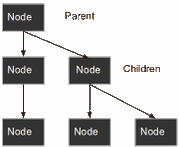
\includegraphics[width=.4\textwidth]{tree}
  \caption{Árvore no Godot.\label{fig:godot-tree} \footnotemark}
\end{figure}
\footnotetext{\url{https://docs.godotengine.org/en/stable/getting_started/step_by_step/scenes_and_nodes.html}}


%% ------------------------------------------------------------------------- %%
\section{Nós}
\label{sec:godot-nos}
 O \textit{Godot} oferece alguns nós específicos para o uso de simulações físicas, fornecendo detecção de colisões entre objetos e diferentes reações caso ocorra o contato. Existem 4 nós específicos para tal função, dependendo do comportamento desejado determinado nó pode ser mais apropriado: \textit{StaticBody2D},  \textit{RigidBody2D}, \textit{KinematicBody2D} e \textit{Area2D}.
 
Todo nó de colisão/física necessita de um filho do tipo \textit{Shape2D} para detectar colisões, pois este fornece a geometria da região que detecta as colisões. Estas podem ocorrer com outros nós ou com as fronteiras da área de jogo. O nó \textit{Area2D} detecta e emite sinais com a presença de outros nós ao seu redor permitindo a programação de uma reação, por exemplo uma esquiva ou animação.

\begin{figure}
  \centering
  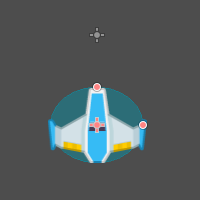
\includegraphics[width=.4\textwidth]{ss/Exemplo area e colisionShape2d.png}
  \caption{Utilizando nós CollisionShape2D e Area2D. Imagem obtida do editor de jogo.\label{fig:area-collision}}
\end{figure}

Na Figura ~\ref{fig:area-collision}, feito para o jogo \textit{Space Shooter}, temos um uso dos nós citados, onde a região em azul sobrepõe a imagem da nave. Esta é um nó do tipo \textit{CollisionShape2D} responsável por detectar colisões com com outros nós, que no jogo são os adversários. A nave por sua vez é um nó do tipo \textit{Area2D} contendo um \textit{sprite} da nave, e quando os nós colidirem, ocorre a emissão de um sinal que terá um comportamento programado, no caso a perda de "vida" do jogador. O conjunto de nós presentes formam uma cena, nesse caso o \textit{Player}.

Nós podem ser agrupados, e o grupo formado atua em conjunto no jogo, conforme a Figura \ref{fig:godot-tree}. O \textit{Tower Defense} e o \textit{SpaceShooter} se aproveitaram de tal característica para a geração dos inimigos e gerenciamento das ondas.

%% ------------------------------------------------------------------------- %%
\section{Sinais}
\label{sec:godot-sinais}

O \textit{Godot} fornece um sistema de sinais, emitidos e detectados por nós, pré-definidos pelo \textit{engine} ou customizados pelo desenvolvedor, que podem servir de gatilhos ou conexões para outras funções em outros nós dentro da hierarquia fornecida pela árvore da cena. As características dos sinais permitem sua utilização em botões na interface, ações em colisões entre nós, entre outras possibilidades.


%% ------------------------------------------------------------------------- %%
\section{Cena}
\label{sec:godot-cena}

A cena no \textit{Godot} é composta de nós organizados segundo uma hierarquia de árvore, onde um nó é a raiz, e seus filhos, que podem ser pais de outros nós, sempre controlados pelo nó raiz, conforme a Figura \ref{fig:scene-tree}, cena feita para o jogo \textit{Space Shooter}. Cenas são objetos independentes, podendo representar somente um elemento do jogo - por exemplo os inimigos, o jogador - ou partes completas dele - como um menu, uma fase.

%% https://docs.godotengine.org/en/stable/getting_started/step_by_step/scenes_and_nodes.html
\begin{figure}
  \centering
  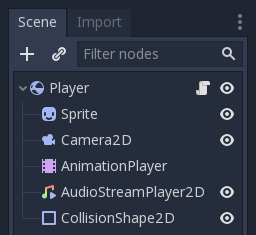
\includegraphics[width=.5\textwidth]{scene_tree_example}
  \caption{Árvore formada por nós no Godot. Em Player um ícone indica a presença de um script vinculado ao nó. Imagem obtida da documentação em \url{https://docs.godotengine.org/en/stable/getting_started/step_by_step/scenes_and_nodes.html}\label{fig:scene-tree}}
\end{figure}



%% ------------------------------------------------------------------------- %%
\section{Instanciação}
\label{sec:godot-instancia}

As cenas de um jogo podem ser inicializadas como objetos filhos de uma outra cena, formando uma instância. Este recurso é usado frequentemente nos jogos desenvolvidos, no \textit{Tower Defense} a fase gera instâncias das cenas das torres e dos inimigos, no \textit{Space Shooter} são instanciados o jogador e os asteróides. As instanciações são feitas de maneira dinâmica durante o jogo, sendo carregadas pelos \textit{scripts} e esperando o \textit{input} do jogador, para a instanciação de um novo objeto que é inserido na árvore de execução. É possível observar o uso da instanciação na Figura \ref{fig:instancia-tiro}, onde a partir do \textit{input} do jogador, projeteis são postos na cena em execução. Cada projetil é uma instanciação, ou objeto, de uma cena feita anteriormente para ser os tiros vistos no jogo.

\begin{figure}
  \centering
  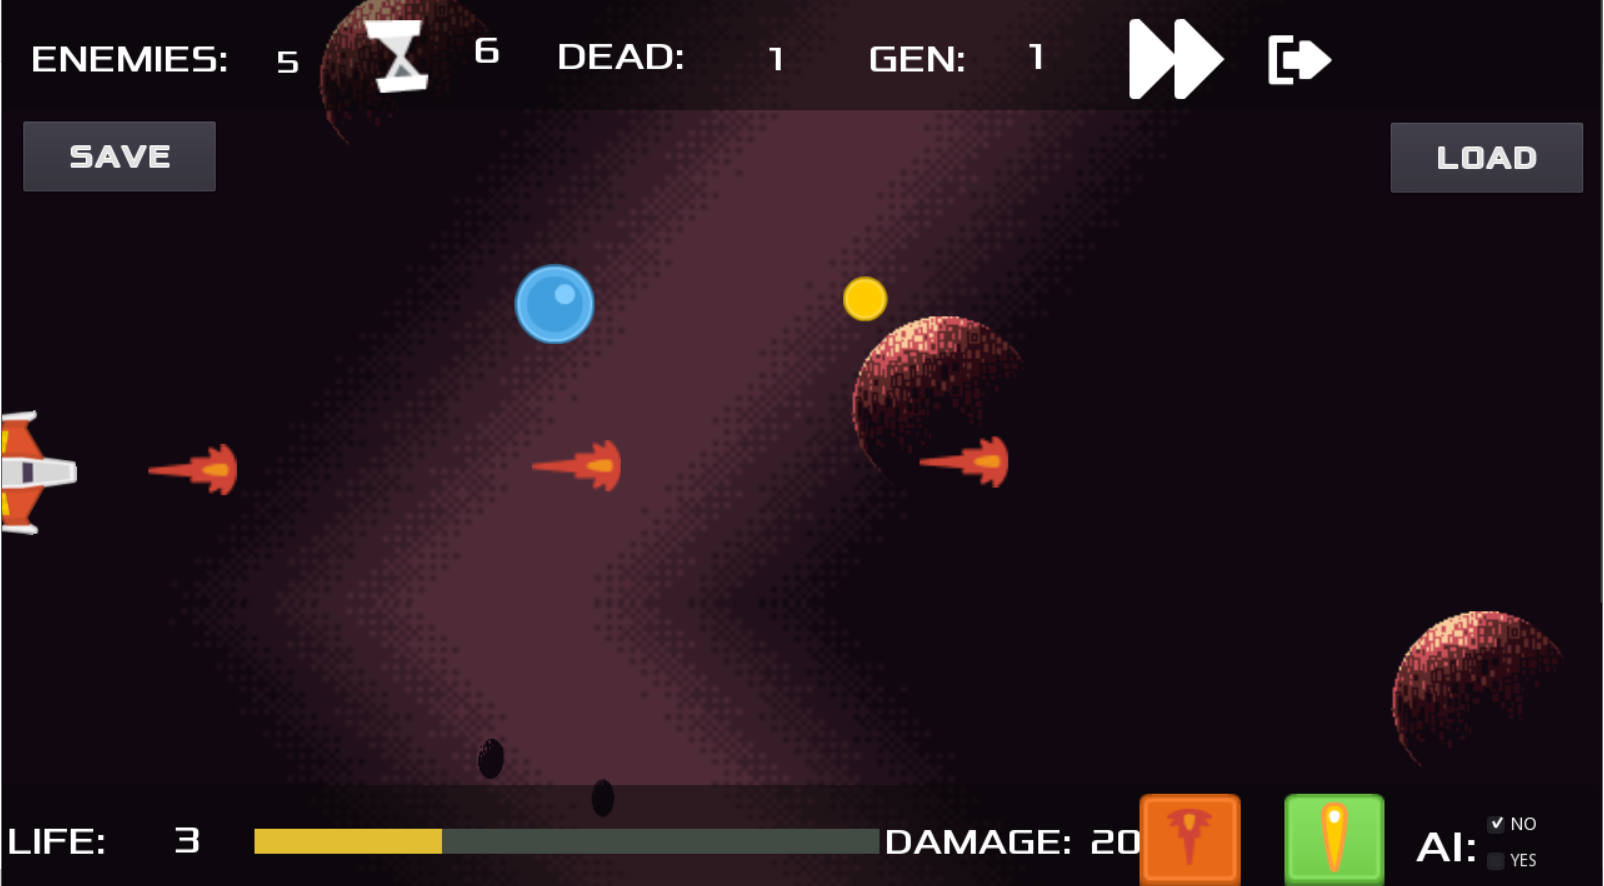
\includegraphics[width=.8\textwidth]{ss/instanciao tiros ss.png}
  \caption{Instanciação de tiros no Space Shooter. Imagem retirada do próprio jogo.\label{fig:instancia-tiro}}
\end{figure}


%% ------------------------------------------------------------------------- %%
\section{Singletons}
\label{sec:godot-singleton}

\textit{Singletons} fornecem a possibilidade de acesso global a métodos e variáveis de outras classes no \textit{Godot}. Semelhante aos sinais, os \textit{singletons} oferecem comunicação entre cenas distintas, relevantes no projeto pois permitiu a implementação do algoritmo genético, que necessita de acesso a diversas variáveis dos jogos, como os inimigos, dano causado, entre outros.

%% ------------------------------------------------------------------------- %%
\section{GDscript}
\label{sec:godot-gdscript}

% Recomendação Will: juntar paragrafos.

Os \textit{scripts} citados são escritos em \textit{GDscript}, linguagem de programação dinâmica de alto nível desenvolvida especificamente para a \textit{Godot Engine}, similar a linguagem de programação \textit{Python} e \textit{Lua}, porém com otimizações e tipos de dados específicos, altamente integrado à própria \textit{engine}\citep{godot-faq}. O editor fornecido integra diversas funcionalidades de um ambiente de desenvolvimento avançado em sua interface, como editor visual 2D e 3D, editor de texto, conexões de sinais, depurador, visualização da árvore de execução durante o desenvolvimento e em tempo real durante a execução, que facilitam o início da produção de jogos.

%% ------------------------------------------------------------------------- %%
\section{Desenvolvimento dos jogos}
\label{sec:desenvolvimento}


% Mencionar o uso de licenças abertas
Para facilitar a familiarização com o ambiente de desenvolvimento e acelerar o foco no algoritmo genético, foram utilizados diversos recursos disponíveis para a produção dos jogos. Desde repositórios de \textit{sprites} como \citet{Kenny_sprites} a tutoriais de \textit{Godot}, sendo o \textit{Space Shooter} baseado no tutorial de \citet{Godot_Linietsy}, disponível na documentação da \textit{engine}, enquanto o \textit{Tower Defense} foi baseado no tutorial disponibilizado pelo \citet{GameDevelopmentCenter21:tdtutorial}. Tanto \citet{Kenny_sprites} como \citet{Godot_Linietsy} possuem licenças que permitem o uso publico ou equivalente, além de serem gratuitas.  
